\section{Designing an Android App (George)}
\label{sec:android-george}
In this section of the report about designing an Android app with the ``Android Developer Tools'' (ADT) software, there will not be any coding guidance on the basics of Java nor XML. As such, any examples discussed or shown will either have a short explanation or will be simple enough to assume the functionality of the code is evident. The ADT software is used in this project as it facilitates the balance in a simple to use package yet includes more detailed app functionality (such as accessing the sound recorder's buffer). There are many other Android app developing software packages, but none achieve this balance as well. For example the ``MIT app inventor'' provides basic building blocks for an app but limits the customisation of the code that is an essential element for our audio processing. ``appsgeyser.com'' is even simpler in providing an app interface for a pre-existing website. However we have decided not to use a web-based approach due to the extra complications from patient security and limitations in excessive data usage in streaming audio to a website.
\subsection{XML and Java sides of ADT}
The ``Android Developer Tools'' software has a simple architecture for basic apps, which uses XML code to create the user interface of buttons and graphics, and Java code to describe to the phone what each of these items in the XML code does\cite[p.~22]{lee2011beg}. So for any page of the phone app, there is an XML code called the ``layout'' with an associated set of Java instructions called a Java ``activity''. Whilst it is intuitively easier to consider a visual layout with instructions behind each section, the programming design works much more naturally the other way around, with the Java activity dictating the layout. For this particular app, we need four pages in total. Therefore we need to create a total of four Java activities to describe each page, and each one of these will call an XML layout to attach various commands to.
\subsection{XML IDs}
Each interactive item of the XML layout will have a unique ID, and the Java code will directly link an object to this, which can then be used in the functionality instructions. The following code first assigns the XML button ID ``btn\_analyse'' to a Java button object called ``btnAnalyse'', then informs the phone to carry out the task ``startAnalyseActivity()'' when it detects that the button has been pressed.
\newpage
\begin{lstlisting}
btnAnalyse = (Button) findViewById(R.id.btn_analyse);
btnAnalyse.setOnClickListener(new View.OnClickListener() {
public void onClick(View v) {
startAnalyseActivity();
          }
    });
\end{lstlisting}
Our application uses a minimalistic interface and as such there are few XML IDs to work with. Regardless, a convention was established such that each object is labeled by it's type followed by an underscore, then it's unique name (for example btn\_analyse as above).
\subsection{Methods}
The task ``startAnalyseActivity()'' used in the example above is known as a ``method'' in Java code and is a set of code instructions grouped together under a single name. Not only does this make the code clearer to understand, it also allows repeated sections of code to be called much more simply: just contain all the repeated parts under one method and call that method each time. For these reasons, code for each part of the application functionality is contained in separate methods.
\subsection{Java and android libraries}
The person writing the app is not expected to write machine level code for the smart phone and the ADT provides a large array of building blocks for both Java and Android based coding which are contained in ``class libraries'' which must be imported at the start of each activity\cite[p.~126]{knudsen2011beg}. For example, the ``Android.media.AudioRecord'' library is needed to use the phone's built in microphone, and it provides simple inbuilt methods such as ``startRecording()'' and ``stop()''. Further details of this particularly important library will be discussed later.
\subsection{Structure of an Activity}
Each activity can be divided down into several key blocks that can be explained in the chronological order in which they are seen in the code:
\begin{enumerate}
\item Importing the necessary libraries of methods
\item Declaring the whole activity to create it
\item Declaring any variables and objects that the activity uses
\item Creating the onCreate() task upon which the activity starts running, and in which the core instructions and external methods are called
\item Defining any extra methods used, with their code detailed inside
\end{enumerate}
\subsection{XML writing}
Again, it is not within the scope of this report to comprehensively explain how to code XML, but the XML code is largely very clear to understand and well labelled. The ``Android Developer Tools'' software allows the user to directly edit the XML code, and to also view and edit the layout from a graphical ``preview'' layout (see Figure \ref{fig:xmlPages}). Note that editing either one of these will update the other in real time. Each object is defined in a block enclosed by \verb!<! and \verb!/>!  and must contain it's own ID definition as a minimum. The app's theme will dictate a large set of default values for any object parameter, so only the physical size and details unique to each object need to be added. This might include unique text for a button or a variation in font for some text -- all of which are edited under very clear labels such as ``android:fontFamily=\dots''.
\begin{figure}[ht!]
		\centering
			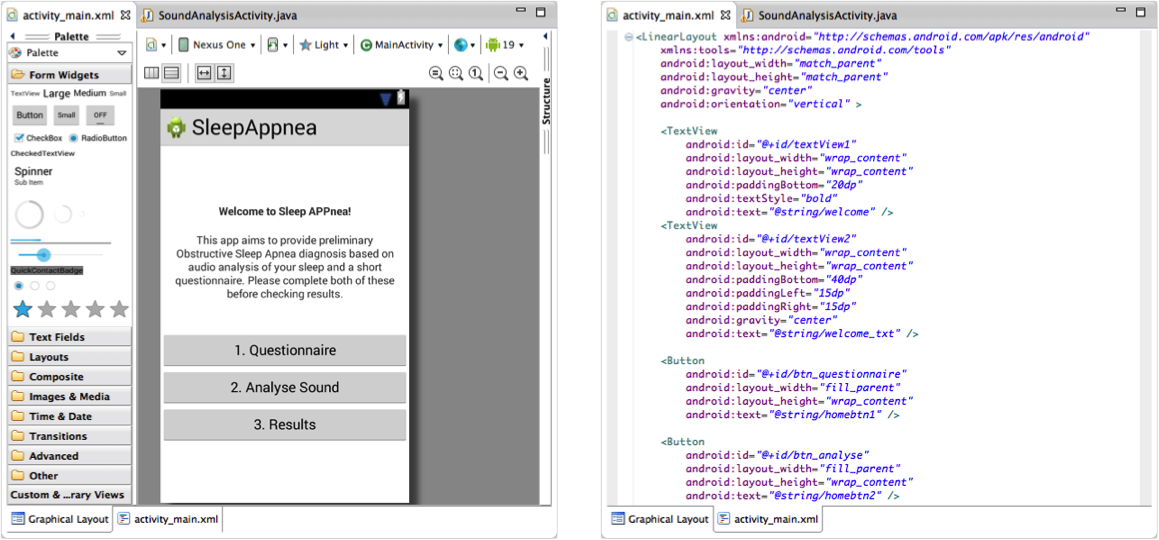
\includegraphics[width=.9\textwidth]{drawings/XML_page.png}
		\caption{The graphical and XML code view of the same User Interface}
		\label{fig:xmlPages}
	\end{figure}
\subsection{XML layouts}
The overall page layout has two main formats: linear layout and relative layout. Relative layout requires each object's relative position to be labelled in reference to at least one other object with a fixed location and allows objects to be placed alongside each other as well as above and below (effectively two dimensions of freedom)\cite[p.~126]{lee2011beg}. Linear layout is simpler and more constrained in that the objects will be placed in the order they appear in the XML code in one dimension. For this application, linear layout is suitable. Other useful tools here include ``\textless ScrollView/\textgreater'' which allows all objects within it to be viewed as a scrollable page. This was used on the questionnaire to prevent the questions becoming too small to be readable. It can also be used internally to scroll a subset of objects rather than the whole page.
\subsection{Further XML details}
When defining an object's size, it's useful to use adaptable sizes to ensure good results on all devices and screen sizes (as opposed to a set height of 10px for example, which could look small on a tablet but large on a small phone). The two options here are FILL\_PARENT, which makes the object as wide as the object it's contained in, and WRAP\_CONTENT, which makes the object as wide as necessary to contain all of its components. Using the example of a button width inside an empty android page, FILL\_PARENT would make the button as wide as the screen, and WRAP\_CONTENT would make the button wide enough to include all the button text.
\subsection{Handling Strings}
When creating buttons and other features with text on, the text should be stored in the separate file in ``res/values/strings.xml'' instead of ‘hardcoding' it directly into the XML code. Whilst it is less of an issue on a small-scale project such as this, it can become increasingly difficult to find where to change particular items of text in larger projects. Instead we label each part of text from the strings file and reference this ID where it is needed in the code. Then we can quickly find where to change any text in future, or perhaps reuse the same text in multiple buttons or other applications.
\subsection{Java Techniques}
Sharing data between activities can be achieved with a basic technique called ``SharedPreferences'' which stores any required variable locally in the app\cite{android2014sp}. As with many techniques, it requires importing its own class from the android library, and vitally requires the command ``editor.commit()'' to save the changes before finishing. It is utilised in this application to store the received information from the questionnaire. By restoring the previous stored settings upon the app initialisation, the questionnaire results are then stored on a more permanent basis (I.E when the application has been closed and reopened).
\begin{figure}[ht!]
		\centering
			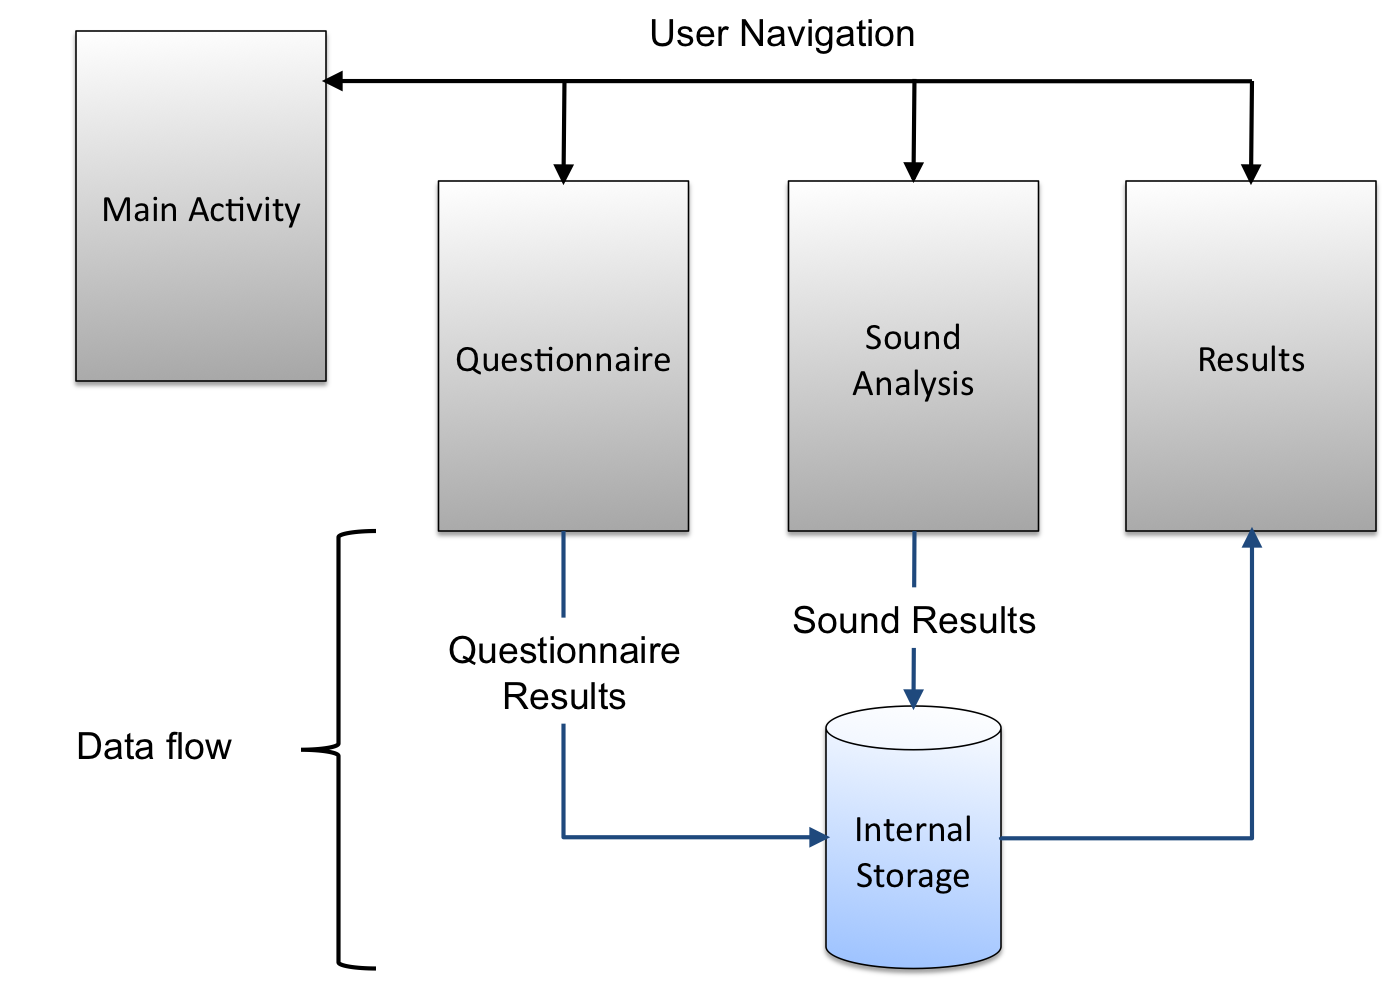
\includegraphics[width=.9\textwidth]{drawings/Data_Structure.png}
		\caption{``SharedPreferences'' utilized to distribute data to the results activity}
		\label{fig:dataStructure}
	\end{figure}

	 Changing from one activity to another is done using a class called ``Intent'' which is effectively setting up a requirement for something to happen. In this case the intent will provide the details of the activity to be launched. A button press might then call ``startActivity(intent)'' which will launch whatever the original intent requested. In this way it can be used as an independent launching mechanism as it is not aware of the details of the intent nor is the intent solely aimed at one target. For example, multiple buttons can launch one action, all acting as effective triggers. In this application, intents are primarily used to launch new activities.

	 When starting multiple activities, care needs to be taken as to how and when previous activities are closed. Whist it might seem to make sense to have the home page close upon opening a new window, this posed a subtle bug in practice. The pressing of two activity-launching buttons simultaneously causes both of them to open and this is not a significant issue. However, pressing the back button in this format requires launching the ``home page'' again. Therefore upon exiting one page, a residual page is left open behind the current home page, and upon a few repetitions of this, the app will quickly be running several pages simultaneously. Without exploring in too much depth how to make each activity-launching button press a unique event (such as a mutex-like control), the simplest solution in this case was to allow up to three of the new activity pages to open simultaneously and leave the ``home page'' unclosed. This limits the total possible number of pages open to four. This is a very unlikely event, and is easily remedied by pressing the back button.

	 ``RadioGroup'' buttons are used in the questionnaire section of the app. These provide the advantages of never leaving a blank answer and being instantly comprehendible to any user. Similarly to the buttons, each one has a unique ID to be linked with the Java activity, but they also have unique IDs for each possible selection. The selected answers can then be acted upon by `if' statements using:
\begin{lstlisting}
if (radioOne.getCheckedRadioButtonId() == R.id.radioY1)
 	 { /* Do action corresponding to yes (answer is radioY1) */ } 
  else
 	 { /* Do action corresponding to no (answer is not radioY1) */}
\end{lstlisting}
\subsection{Initialising AudioRecord}
It is worth looking in further detail at the AudioRecord android class that we use for the audio input. The initialisation of ``new AudioRecord()'' uses five parameters, which are explained below:
\begin{itemize}
\item ``audioSource'' should be set to ``1'' to default to the inbuilt microphone
\item ``sampleRateInHz'' should be set to ``44100'' to guarantee functionality on all devices, however a much lower sample rate would be preferable for the basic application here, and a solution to this is described below.
\item ``channelConfig'' should be set to `16' for recording sound in MONO rather than STEREO. 
\item ``audioFormat'' should be set to `2' for PCM 16bit or `3' for PCM 8bit. This application uses 16bit to ensure functionality on the greatest number of devices possible.
\item ``bufferSizeInBytes'' is set using an inbuilt method called ``getMinBufferSize()''. The inputs to this are the same as parameters 2, 3 and 4 in the AudioRecord initialisation.
\end{itemize}
So the initialisation for the application should look as follows:
\begin{lstlisting}
new AudioRecord(1,44100,16,2,getMinBufferSize(44100,16,2));
\end{lstlisting}
In practice, each input is assigned to a variable that is defined at the top of the code for easy modification and better clarity in the code.

 For recording snoring frequencies, a sample rate of as low as 4000Hz would be adequate. The following code solves the earlier discussed issue of minimising the sampling rate. The ``getMinBufferSize()'' is tested on each value added in the for() loop, but as soon as the function returns a positive (hence a valid) bufferSize, the method returns this lowest valid sample rate and ``breaks'' to finish the method.
\begin{lstlisting}
public int getValidSampleRates() {
  int samplerate = 0;
for (int rate : new int[] {8000, 11025, 16000, 22050, 44100}) {
  int bufferSize = AudioRecord.getMinBufferSize(rate, AudioFormat.CHANNEL_CONFIGURATION_DEFAULT, AudioFormat.ENCODING_PCM_16BIT);
if (bufferSize > 0) {
  samplerate = rate;
  break;}
}
return samplerate };
\end{lstlisting}
\subsection{Progress Wheel}
A progress wheel requires two tasks to be carried out simultaneously -- the wheel itself, and the task that has the progress being indicated. This is done with the `AsyncTask' class library that allows a background operation to interact with the user interface element: effectively two threads are running and we can allow the UI thread to be updated from the background task. There are four self-explanatory steps in the asynchronous task called onPreExecute, doInBackground, onProgressUpdate and onPostExecute.

 To use an example in this app, the ``SaveToFileTask'' first calls the progress wheel to show on screen with ``ProgressDialog.show(…)'' in the onPreExecute() step (Figure \ref{fig:loadingData}). It then calls the method ``audioData.saveData(…)'' in the ``doInBackground()'' step. Finally it calls ``progressDialog.dismiss()'' in ``onPostExecute()'' which will clearly indicate that the data has been saved. Note that the ``onProgressUpdate'' step is not used, as we do not have a use for updating the UI whilst running the background task. This might, for example, be used to change the text on the progress wheel to indicate when a second task is being carried out had one been present.
\begin{figure}[ht!]
		\centering
			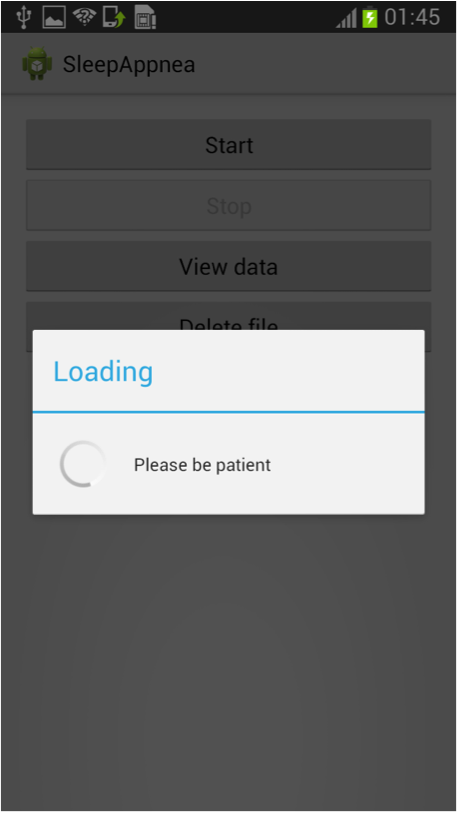
\includegraphics[width=.4\textwidth]{drawings/Loading.png}
		\caption{Use of AsyncTask to update to the UI thread whilst loading data}
		\label{fig:loadingData}
	\end{figure}

\subsection{Other Platforms}
Apple provide their own libraries similar to those in android, that provide quickly usable methods and hardware capability to a developer. The sleep apnea app has suitably simple components that can be recreated on Apple's iOS like for like if required. This section of the report will quickly overview the techniques to do this, but will also detail other available tools and how they might be used more to create a more effective native app in iOS. This section will not detail any code, purely discussion of the available libraries and tools.
\subsection{Xcode}
Xcode is the free software available in the Apple App Store that contains all the necessary prototyping and developing tools to produce an application on iPhone, iPad and Mac. Code can be written in Objective-C, C and a whole multitude of other languages with interpreters to adapt them. Xcode provides an Integrated Development Environment (IDE), compiler with inbuilt ``bug'' finding, an iOS simulator to virtually test the app amongst other things. Similarly to the Android Developer Tools, memory analysis, CPU profiling and general performance tracking is all included. This would provide a very suitable basis to build our app from.
\subsection{AVAudioRecord Library}
The most important library to consider here is the inbuilt capabilities of the audio recording. A handful of the more unique and interesting classes will be discussed here:
\begin{itemize}
\item recordAtTime:forDuration: This flexibility in setting the start time to record and the duration of each recording could be applied for a few things. Firstly the start time could be set such to greatly increase the chance of the user being asleep as the recording starts. It could also be used as a basic way to reduce background noise if, perhaps, the user's sleeping area experienced background noise from parties or traffic until a set time in the evening. Likewise, limiting the duration of the recording could ensure results aren't skewed from noise of waking up and manually turning the app off. The app could select a key range of hours in the night that maximises the probability of apnea detection and minimises the chance of background noise. Note that this could also be manually implemented in the Android version which is discussed later.
\item averagePowerForChannel: This is one of two values provided in the Audio Level Metering section of the library. This could provide a very simple technique to implement a switching state model with perhaps three defined ranges of audio powers. Recording the average power for the channel (in our case there is only one channel in MONO recording) roughly twice per second would provide an array which would accurately reflect the volume of the sleeping user. ``Band two'' would represent the standard snoring volume observed in almost all sufferers of sleep apnea and would be the expected volume level for the user. ``Band one'' would be very low audio power indicative that the sleeper's throat is blocked and an apnea is occurring. ``Band three'' would represent high audio power, interpreted as the loud snorting very commonly experienced after an apneic episode as the sleeper unblocks their throat (see Figure \ref{fig:bandGraph}). Clearly such a monitoring system would produce very small file sizes, which is a very desirable aim in audio recording based software (in this case, audio isn't being saved directly to a file, only monitored for power values). This technique doesn't lend itself well to machine learning techniques due to the lack of precision in the recorded data -- features aren't defined nearly as well as more fully sampled techniques.
\item peakPowerForChannel: This is the other value provided by the Audio Metering section and whilst not being as directly applicable, it could be useful when used in conjunction with averagePowerForChannel. From simple logical reasoning, noise is much harder to detect when the precision of the system is low like the technique suggested above. peakPowerForChannel could therefore be used to calibrate this technique. A short recording of the background noise in controlled quiet conditions could calibrate the allowable background noise for ``band one'' in the above example, whilst the user recording a faked snort sound could provide a rough expectation for the power level at ``band three''. From this, unexpected audio power levels can be rejected or handled differently from the normal operational audio power.
\begin{figure}[ht!]
		\centering
			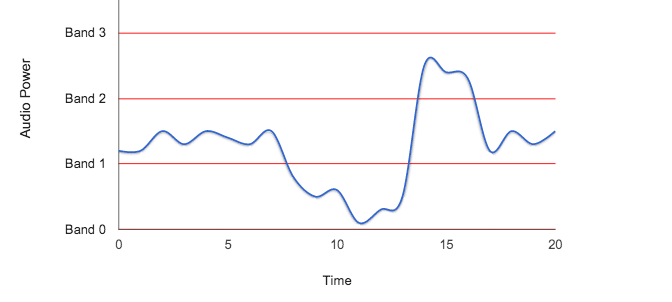
\includegraphics[width=1\textwidth]{drawings/Band_graph.png}
		\caption{Bands 1, 2 and 3 representing an apnea, snoring and an arousal respectively}
		\label{fig:bandGraph}
	\end{figure}
\end{itemize}